\chapter{Event selection} \label{chap:event_selection}
\section{The monophoton signature and background sources} \label{sec:event_selection_backgrounds}
In order to conserve overall \pT, a \zinvg\ event with a high-\pT\ photon (significantly exceeding that of other visible particles in the event)
must have a neutrino pair emitted with a total \vecpT\ of approximately the same magnitude as \vecpTgamma, oriented in an opposing direction\footnote{The \pT's
of the photon and the neutrino pair must exactly cancel if there are no other particles emitted from the same \Pp\Pp\ collision. The photon and neutrinos (as well as
their parent \PZ) have a very low probability of radiating or converting into other particles that would not be correctly associated together by PF.
However, other particles are routinely emitted from the underlying event or from the incoming partons, and while they are typically much softer than the \Pgamma\ and
\Pn's, they can significantly shift the overall \pT\ balance of the \Pgamma--\Pn\Pn\ system.}.
The same is true of the BSM models described in Chap.~\ref{chap:introduction}, with a pair of DM particles or an ADD graviton replacing the neutrino pair.
These BSM particles as well as neutrinos have a very low probability of undergoing any direct, detectable interaction with the CMS experiment, and are instead reconstructed as \MET.
Thus each of these processes gives rise to events with a high-\pT\ photon emerging against a comparable amount of \MET, with no other significant particle emissions.
Events with this signature are said to be in the \textit{monophoton channel}.

The presence of BSM physics would be induced by the observation of a significant excess of observed monophoton events over the expected SM background.
The dominant SM source of monophoton events, with no other particles in the event that could be used to robustly identify it, is the \zinvg\ process.
Since a \zinvg\ event has exactly the same visible signature as a BSM event of the types described above, \zinvg\ is the primary \textit{irreducible} SM background
to BSM searches in the monophoton channel, contributing more than half of the expected SM event yield. The estimation of its expected contribution is therefore of
primary concern in not only the \zinvg\ cross section measurement, but in monophoton BSM searches as well.

Other SM processes have additional visible particles in the event beyond a single high-\pT\ photon. These extra particles make it possible in principle to unambiguously
identify these events as non-\zinvg\ (given a perfect detector and reconstruction algorithm), and so these events constitute the \textit{reducible} background.
The event cleaning cuts in this thesis include a lepton veto that rejects events containing any extra muons or electrons with substantial \pT,
removing a large fraction of this background.
Sometimes particles will escape through small gaps in the detector, be absorbed by some interstitial layer of support structure, or more generally fail to produce
discernible deposits in the detectors that could be reconstructed as PF elements. Even if corresponding PF elements are produced, sometimes an object of one type will
be misreconstructed as one or more objects of another type. If a key identifying particle is misreconstructed or lost, the event may pass a particle-specific veto, but these
events can still often be identified by a relative imbalance in \vecpTgamma\ vs. \vecMET\ introduced by the extra particles.
A series of kinematic cuts are employed to retain only those events in which \vecpTgamma\ and \vecMET\ have magnitudes and directions especially consistent with
\zinvg\ production.

If a \PW\ is produced opposite a \Pgamma, the \PW\ will give rise to substantial \MET\ if it decays into a lepton+neutrino (\wlng). If the lepton is identified, it can be used
to tag the event as having a probable \wlng\ origin, but if the lepton is lost, the event is likely to have a similar kinematic profile to
a \zinvg\ event. Summed over all \ETgamma\ bins, this is the largest single source of background to the \zinvg\ cross section measurement (and second largest source of background
to BSM searches), particularly at low \ETgamma, contributing just under 20\% of the total expected SM event yield.
The need for precise \wlng\ background estimation, and for precise \zinvg\ background estimation in the context of BSM searches, motivates the use of transfer
factors (sec.~\ref{sec:signal_extraction_SM}, \ref{sec:signal_extraction_DM_ADD}) linking the signal regions to various control regions defined in this chapter.

An electron that leaves deposits
in the ECAL but with no matching track identified in the inner tracker is likely to be reconstructed as a photon. These electron faking photon events are a significant
source of background in the monophoton channel, primarily due to $\PW \to \Pe\Pn$ where the \MET\ comes from the \Pn. This is the second largest source of overall background to
the \zinvg\ cross section measurement, and the largest source for $\ETgamma > 300\unit{GeV}$. A jet containing high-\pT\ photons from neutral
pion decays can be reconstructed as an isolated photon if PF fails to find matching HCAL deposits from other hadrons in the jet. These jet faking photon events produce a monophoton
signature if the jet emerges opposite a \PZ\ which then decays into neutrinos. Electron fakes and jet fakes contribute about 15\% and about 4\%, respectively, of the total
expected SM event yield in the signal regions.

Jets are composite objects with highly stochastic profiles, and the accurate reconstruction of their transverse momentum depends on the accurate \pT\ or energy reconstruction
of all of their constituent particles. Even after jet energy corrections are applied (and \vecMET\ is correspondingly
rebalanced), the uncertainty on a jet's \pT\ can be 2\% or more. If the jet is aligned with the \vecMET, this uncertainty is translated entirely into \MET\ uncertainty,
and a badly-measured jet \pT\ will result in a correspondingly inaccurate \MET\ value. An event in which a single photon is balanced by one or more jets (\gjets), which ordinarily has
insufficient \MET\ to be selected, can produce a monophoton signature if a jet \pT\ mismeasurement boosts the reconstructed \MET\ by a large amount. Kinematic and jet
cleaning cuts ensure that the \gjets\ background is kept to a small percentage of the expected SM yield in the signal regions.
Other minor sources of SM background include \zllg, $\PV\PV\Pgamma$ ($\PV = \PW,\PZ$), $\PW(\Pmu\Pn)$, $\PW(\Ptau\Pn)$, $t\Pgamma$, and $t\bar{t}\Pgamma$. These generally imitate
a monophoton signature if a lepton is misreconstructed or lost, if a jet has a badly mismeasured \pT, or both. Together, the minor SM backgrounds contribute about 10\% of the total
expected SM yield in the signal regions.

A beam halo muon that leaves deposits in the ECAL can be reconstructed as a PF photon, particularly if those deposits are left in a region of little surrounding activity.
The vast majority of collision events do not have a \pT\ imbalance of tens of \unit{GeV} or more, and so there is an extremely high probability that the reconstructed \MET\ will
have almost exactly the same magnitude and opposite direction as that of the beam halo photon. The same reasoning applies to events with spikes, with the result being that beam
halo and spike photon events are very likely to be selected as monophoton events unless reliable photon identification criteria can be applied.

The following sections describe the cuts that define the various signal and control regions used in this analysis. All cuts are employed in all regions unless
otherwise stated.

\section{Trigger and \texorpdfstring{\MET}{pTmiss} filters} \label{sec:event_selection_trigger_METfilters}
Every observed event must first pass a specific HLT path in order to be examined in this analysis. This path rejects the millions of collision events that have no observable
monophoton characteristics, by requiring there to be at least one reconstructed photon passing minimal quality criteria.
The low-\pTgamma\ phase space has been explored by other experiments (Chap.~\ref{chap:introduction}), and the high collision energy of the LHC introduces a significant
level of relatively high-\pT\ background activity that diminishes the statistical value of low-\pTgamma\ events.
Thus, a minimum \ETgamma\ cut of 165\unit{GeV} was chosen for the monophoton HLT path.
Furthermore, candidate photons must have an $H/E$ ratio (sec.~\ref{sec:reconstruction_egamma}) less than 0.10.
Online photon reconstruction implemented in the HLT is less precise than the full offline reconstruction performed after the data has been selected and stored,
so cuts on the HLT photon are less restrictive than the final cuts applied on the offline photon.

The selection efficiency of this HLT path was estimated in observed data by first selecting events passing a different set of triggers (requiring only a jet with \pT\ greater than
either 60, 80, or 140\unit{GeV}), applying all analysis cuts, and finally checking the fractinon of these events that passes the monophoton trigger.
The efficiency as a function of \ETgamma\ is shown in Fig.~\ref{fig:trigger_efficiency}.
A linear fit to the efficiency for $\ETgamma > 175\unit{GeV}$ yields a slope of $-0.00004395$ and a  $y$-intercept of $1.002$. The impact of the trigger was estimated
in simulated MC events by multiplying each event by a weight equal to the value of the linear fit at \ETgamma. In order to estimate the uncertainty on the expected
SM background corresponding to trigger inefficiency, the uncertainties in the linear fit parameters are propagated through this event weight.

\begin{figure}[hbtp]
  \begin{center}
    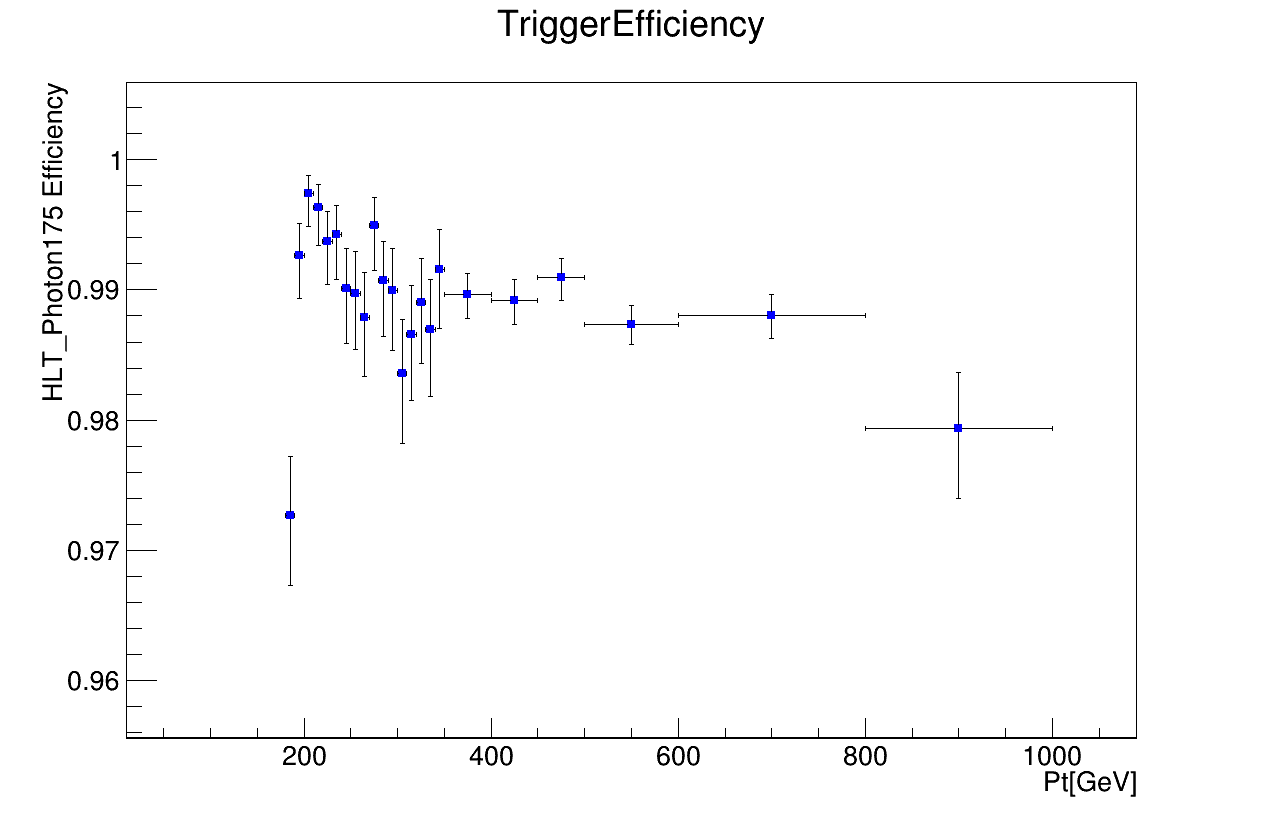
\includegraphics[width=0.75\textwidth]{Figures/triggereff_zoom.png}
    \caption{
    Absolute trigger efficiency of the monophoton HLT path HLT\_Photon165\_HE10.
    }
    \label{fig:trigger_efficiency}
  \end{center}
\end{figure}

In addition to passing the HLT path, every event must pass a set of \MET\ filters which guard against clearly spurious sources of \MET. If during some collision event
a detector element is not performing according to nominal specifications, e.g. because it is malfunctioning or turned off, the resulting reconstructed energy balance will
not be a reliable indicator of its true value. Events are rejected if they have a known instrumental issue of this sort.

\section{Photon} \label{sec:event_selection_photon}
Preliminary studies indicated that an \ETgamma\ cut of 175\unit{GeV} (along with a \MET\ cut of 170\unit{GeV}) would result in maximal discovery potential across
multiple BSM scenarios. Every event must contain at least one reconstructed photon with at least this much \ETgamma. Both here and below,
\ETgamma\ refers to the photon's raw supercluster \ET, for the reasons given in sec.~\ref{sec:reconstruction_egamma}. The photon candidate with the highest
\ETgamma\ is called the \textit{leading photon}.

Due to the high radiation fluences at high $|\eta|$, and the resulting use of VPTs instead of APDs, measurements of \ETgamma\ in the endcaps are significantly less precise
than those in the barrel. This reduces the statistical value of using EE photons, and we confirmed that their inclusion would not significantly alter the final results
of our analyses. Furthermore, the non-projective layout of EE crystals makes it much less straightforward to identify fake photons stemming from beam halo.
The leading photon must therefore lie within the barrel acceptance. To avoid energy leakage out of the barrel edges, as well as a layer of instrumentation partially
covering the outermost EB crystals, the leading photon must lie within $|\eta| < 1.4442$.

A photon originating from a neutral pion in a jet will tend to be accompanied by various other particles in a jet-sized $\Delta R$ cone. For a given type of PF particle
(photons, charged hadrons, or neutral hadrons), the corresponding \textit{isolation} is defined to be the sum of particle energies for all particles of that type
within a $\Delta R < 0.3$ cone around the photon. A large isolation value indicates that the photon is likely to be fake.
In most CMS analyses, charged hadron isolation only considers charged hadrons with tracks linked to the leading PV. However,
the leading PV is chosen based on the sum of track $\pT^{2}$ of all tracks (and track \MET) linked to the PV, and monophoton vertices do not necessarily have charged tracks
with any substantial amount of \pT. The \textit{max charged hadron isolation}, defined to be the maximum value of charged hadron isolation with respect to any vertex in the event,
gives a more robust estimate of charged hadron activity that is more suitable for monophoton events.

Calculation of a given type of isolation sum begins by summing the energies of all PF particles of that type near the photon. As pileup increases, an increasing number of PF particles
will be reconstructed out of pileup events, and an increasing amount of isolation energy will correspond to pileup energy. The energy carried by particles of a given type is observed to vary
linearly as a function of the estimated pileup energy density $\rho$. The slope of this linear dependence has dimensions of area and is called the \textit{effective area} ($A_{eff}$)
corresponding to particles of a given type. Subtracting $\rho{*}A_{eff}$ removes the pileup energy dependence from an isolation sum, leaving the \textit{corrected isolation}.

The CMS monophoton group developed a custom monophoton ID for 2016 analyses, based on five variables: $H/E$, photon isolation, max charged isolation, neutral isolation, and the photon shower shape
variable \sieie\ defined by
\begin{equation}
\begin{gathered}
\begin{aligned}
\sieie &= \sqrt{\frac{\sum_{i\in5{\times}5} w_{i}(i\eta_{i} - {\bar{i\eta}}_{5{\times}5})^{2}}{\sum_{i\in5{\times}5} w_{i}}}\\
            w_{i} &= 4.7 + \ln{(E_{i} / E_{5{\times}5})}
\end{aligned}
\end{gathered}
\label{eq:sieie}
\end{equation}
where the sums run over the $5{\times}5$ crystal array centered on the supercluster seed, $E_{i}$ is the energy of crystal $i$, $E_{5{\times}5}$ is the sum of all crystal energies
in the $5{\times}5$ array, and (in the barrel) $i\eta_{i} - {\bar{i\eta}}_{5{\times}5}$ is the number of $\eta$-rows of separation between crystal $i$ and the center of the $5{\times}5$ array\footnote{The value
of 4.7 is essentially arbitrary. It scales \sieie\ so that a typical real photon in the barrel has $0.005 < \sieie < 0.011$.}. This variable
describes the energy spread of a photon's ECAL cluster---the more spread out a cluster is, the larger the value of \sieie.
The cuts defining the monophoton ID are listed in Table~\ref{tab:photonID}. The numerical values in these cuts were tuned to retain minimal jet fake events while retaining 80\% of
real \zinvg\ events in any $\ETgamma$ range above 175\unit{GeV}. Table~\ref{tab:effective_areas} lists the $A_{eff}$ values used to compute the corrected isolation.

\begin{table}
\centering
\begin{tabular}{ c|c }
\hline
Variable & Cut value \\
\hline
$H/E$ & 0.0260 \\
\sieie & 0.01040 \\
corr.\ max charged hadron iso.  & 1.146 \\
corr.\ neutral hadron iso. & $2.792 + 0.0112{*}\ETgamma + 0.000028{*}{\ETgamma}^{2}$ \\
corr.\ photon iso.  & $2.176 + 0.0043{*}\ETgamma$ \\
\hline
\end{tabular}
\caption{Cuts defining the 2016 monophoton ID, applicable to photons in the barrel.
A cut is passed if the expression in the left column is less than the value in the right column.
The effective areas used to compute the corrected isolation values are listed in Table~\ref{tab:effective_areas}.}
\label{tab:photonID}
\end{table}

\begin{table}
\centering
\begin{tabular}{ ccc }
\hline
Type of isolation & $|\eta| < 1.0$ & $1.0 < |\eta| < 1.479$ \\
\hline
max charged hadron & 0.01064 & 0.1026 \\
neutral hadron & 0.0597 & 0.0807 \\
photon & 0.1210 & 0.1107 \\
\hline
\end{tabular}
\caption{Effective areas used in the 2016 monophoton ID.}
\label{tab:effective_areas}
\end{table}

The ID defined by the cuts in Table~\ref{tab:photonID} does not take into account whether or not the particle being ID'd has a corresponding track, relying instead solely on the distribution
of energy in the calorimeters in conjunction with the level of ``pollution'' of surrounding particles. The shower profiles of electrons are extremely similar to those of photons, and in principle
this ID works approximately as effectively to select real electrons, if track information is not taken into account. We obtain an estimate of the photon efficiency of this ID by examining its
efficiency for electrons, using the high cross-section $\PZ(\Pe\Pe)$ process as a ``standard candle'' for the \textit{tag-and-probe} method~\cite{ref:CMS-PAS-EGM-07-001}. An electron passing
tight ID requirements is identified as a tag electron, and a second electron passing much looser requirements is called the probe electron. The identity of the probe electron is reinforced by
its consistency with the $\PZ(\Pe\Pe)$ hypothesis: the event is selected as a good tag-and-probe event if the invariant mass of the tag--probe pair is close to the \PZ\ mass, and the background
of non-$\PZ(\Pe\Pe)$ events is estimated (and then subtracted out) by fitting an expected $\PZ(\Pe\Pe)$ shape along with an expected background shape to the invariant mass distribution.

In this case, the probe electron is examined to see if it passes the monophoton ID. The number of probes passing the ID, divided by the total number of probes examined, gives an estimate of the efficiency
of the monophoton ID. The photon ID efficiency was estimated using both observed and simulated data. The ratio of the two sets of efficiency measurements is shown in Fig.~\ref{fig:phoID_SF}.
Fitting a horizontal line to the figure, the ratio of the data efficiency to the MC efficiency is estimated to be $1.002 \pm 0.007$. This \textit{efficiency scale factor} is applied as an event
weight to all simulated events, and the uncertainty of 0.007 is propagated to the final analysis results through this weight.

\begin{figure}[hbtp]
  \begin{center}
    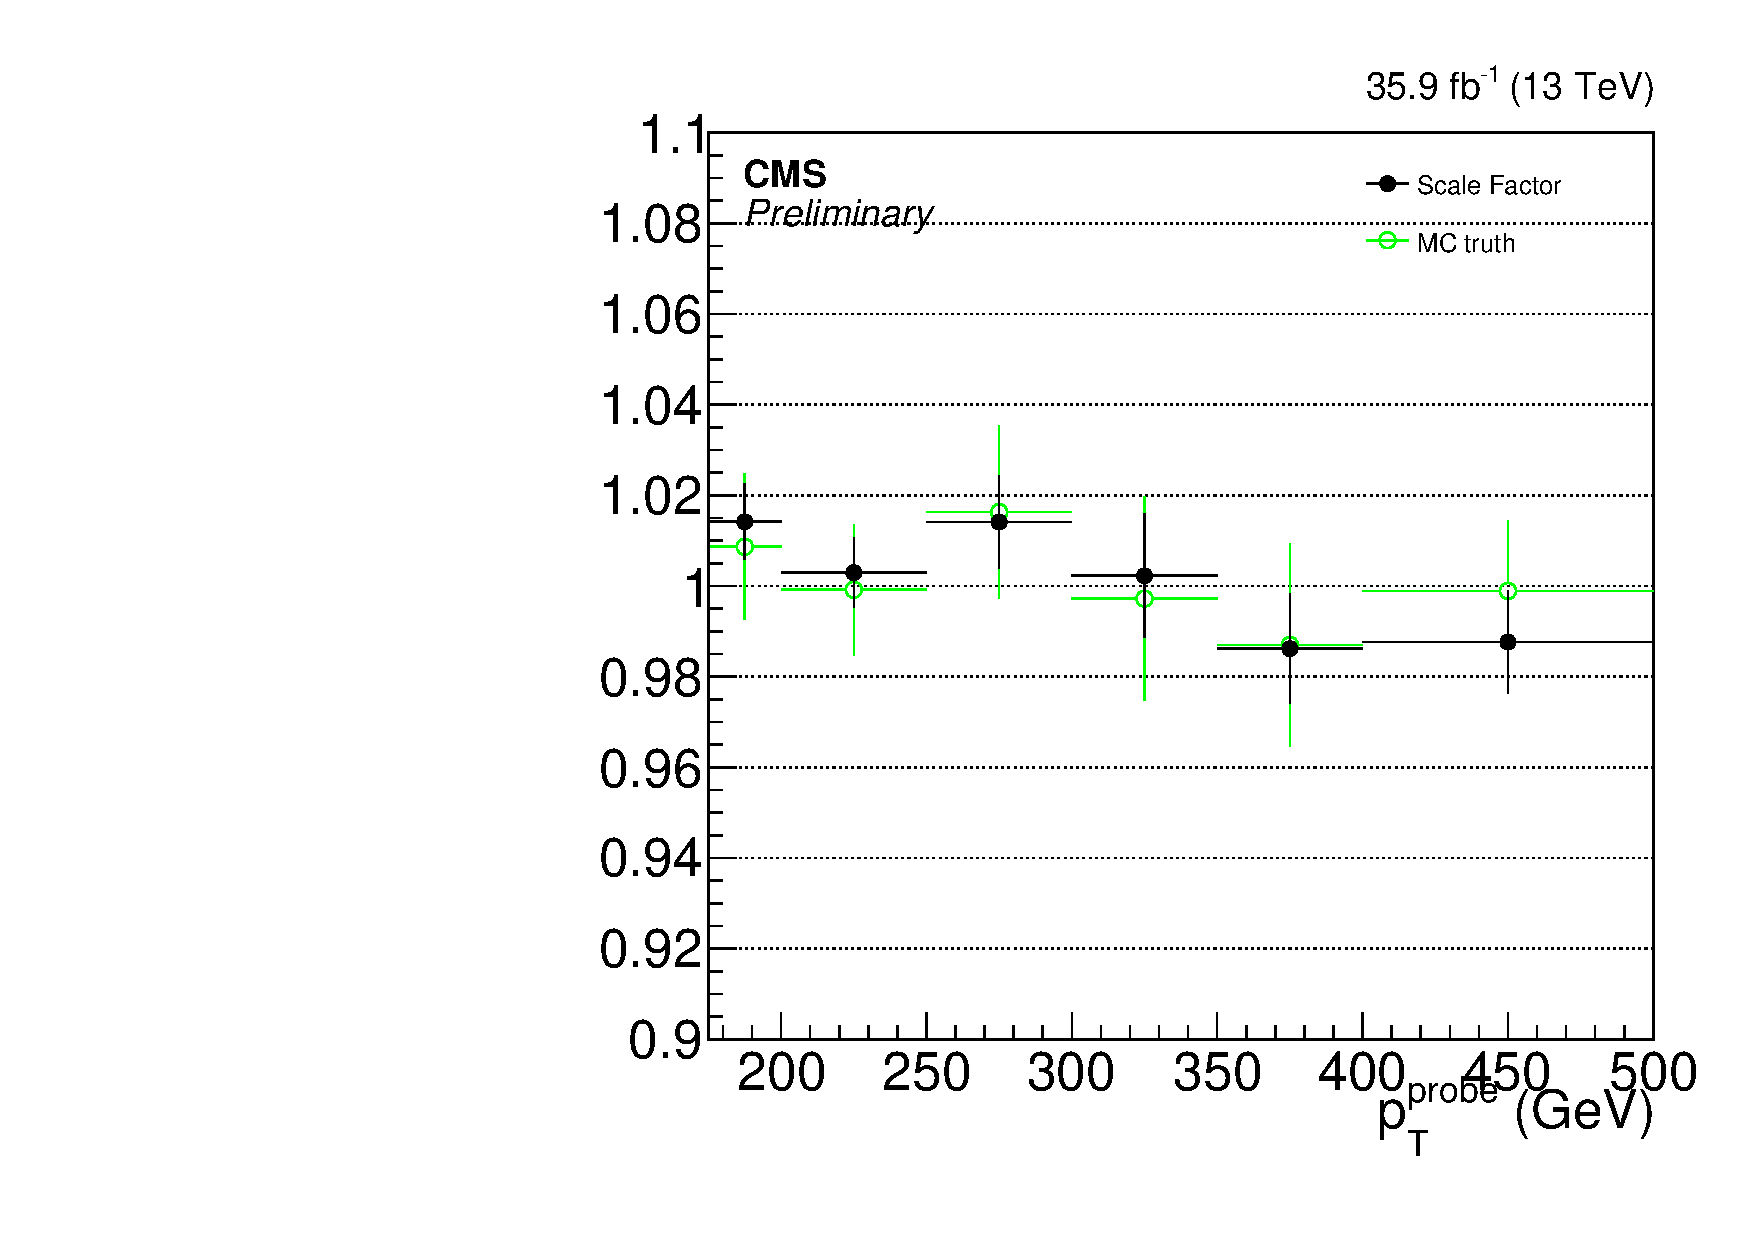
\includegraphics[width=0.65\textwidth]{Figures/phoID_SF.pdf}
    \caption{
    Efficiency scale factors for the monophoton ID requirements of Table~\ref{tab:photonID}, binned in terms of the probe electron \pT. The black points are obtained with the tag-and-probe method in
    both observed and simulated events. For the green points, the simulated efficiencies were instead calculated by geometrically matching the reconstructed electrons to generated electrons,
    and then dividing the number of matched electrons passing the ID by the total number of matched electrons. The two separate methods of computing the MC efficiency yield
    efficiency scale factors that are consistent within uncertainties in every \pT\ bin. The overall photon ID efficiency scale factor is obtained by fitting a horizontal line to this plot.
    }
    \label{fig:phoID_SF}
  \end{center}
\end{figure}

An electron may fake a photon if it has a well-reconstructed ECAL supercluster but a poorly-reconstructed track. A track may be reconstructed poorly if the electron failed to leave very many hits,
or if the hits it left were incorrectly assembled by the tracking algorithm. In these cases, the electron may still have left a \textit{pixel seed} consisting of at least two hits in the pixel tracker
with an inferred trajectory consistent with the supercluster~\cite{ref:1748-0221/10/08/P08010}. To remove as much of this background as possible, an event is only retained if the leading photon does
not have a matching pixel seed.

A real high-\pT\ photon essentially never has a \sieie\ value of 0.001 or less. Such a value is consistent with a single crystal having all or nearly all of the energy of the
reconstructed photon, which is much more consistent with a spike than with a real photon. The same applies to a \sipip\ value of 0.001 or less, where \sipip\ is
defined in a similar way as \sieie. In order to clean out spikes, an event is only retained if the leading photon has $\sieie > 0.001$ and $\sipip > 0.001$.

A beam halo muon impinging on EB will be traveling roughly parallel to the beamline, and can therefore leave energy deposits in a line of EB crystals extended in $\eta$ and narrow in $\phi$.
The sum of EB crystal energies in lines consistent with a beam halo muon, for any such lines passing through a given photon seed,
is the \textit{halo total energy} $E^\mathrm{halo}$. An event is only retained if $E^\mathrm{halo} < 4.9\unit{GeV}$.

Most hard \zinvg\ events occur within 3\unit{ns} of the nominal bunch collision time. In contrast, spikes tend to arrive more than 10\unit{ns} early, as described in sec.~\ref{sec:LHCCMS_CMS_ECAL}.
Beam halo accompanies the bunches and reaches the center of CMS just as the bunches collide. Photons from the bunch collision then take an additional few nanoseconds to reach ECAL,
with the net result being that beam halo tends to be reconstructed a few nanoseconds early. A photon arrival time cut of $|t| < 3\unit{ns}$ helps to further suppress these sources of background.

The efficiency of the preceding cuts (following the monophoton ID) is measured in a \gjets-enriched control region, defined by selecting events with at least one jet passing $\pT > 100\unit{GeV}$,
$|\eta| < 2.5$, and passing loose ID criteria. In addition, a $\MET < 60\unit{GeV}$ cut is applied to ensure that this control region is orthogonal to the signal regions. A photon
is selected which passes the monophoton ID cuts, with loosened worst charged iso.\ and \sieie\ requirements in order to be able to perform a template fit on the \sieie\ distribution.
This template fit is used to estimate and then subtract out the number of fake photons in this control region. A real photon template is taken from the \sieie\ distribution of real photons in
simulated \gjets\ events, and a fake photon template is taken from a high-worst-charged-iso. sideband. The templates are cleaned and systematic uncertainties are estimated using methods
very similar to those described in detail in sec.~\ref{sec:background_estimation_jetfake}.

A fit is performed on the observed distribution of all ID'd photons, and then a separate fit is performed on the observed distribution of
all ID'd photons that also pass the pixel seed, spike cleaning, and halo cleaning cuts. Each fit yields its own real photon count, and the ratio of those counts gives the observed efficiency
of the last set of cuts. The efficiency is estimated in simulation by counting the number of gen-matched reconstructed photons passing all cuts and
dividing by the number of photons passing at least the monophoton ID cuts. The ratio of the efficiency estimates in observed and simulated data, shown in Fig.~\ref{fig:pixseed_SF},
gives a second photon efficieny scale factor. Fitting a horizontal line to Fig.~\ref{fig:pixseed_SF} yields a value of $0.984 \pm 0.009$. This value is applied
as an event weight to all simulated data, and the corresponding uncertainty is propagated through this weight to the final results.

\begin{figure}[hbtp]
  \begin{center}
    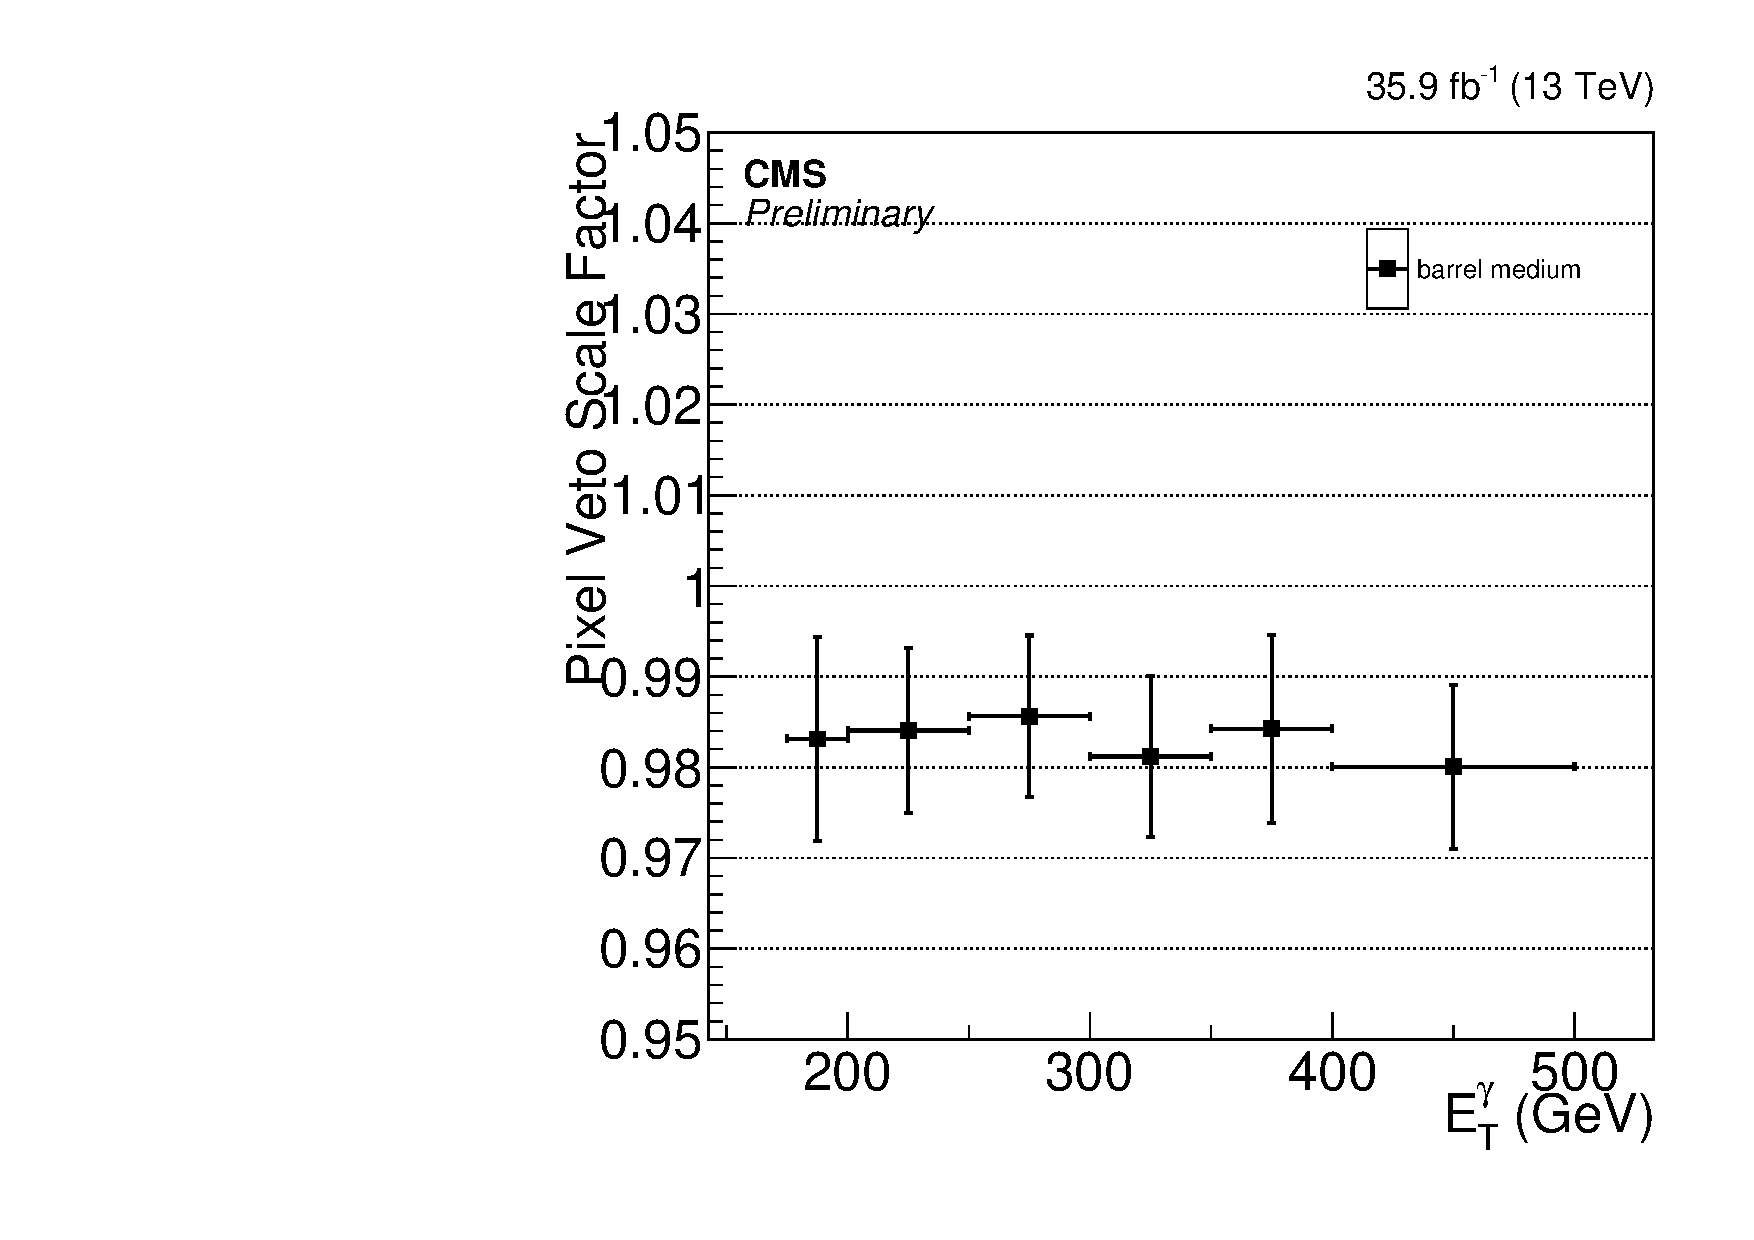
\includegraphics[width=0.65\textwidth]{Figures/pixseed_SF.pdf}
    \caption{
    Efficiency scale factors for the combined pixel seed, spike cleaning, and halo cleaning cuts.
    }
    \label{fig:pixseed_SF}
  \end{center}
\end{figure}

The variable $R_{9}$ is defined as the energy of the $3{\times}3$ crystal array centered on the most energetic crystal in the supercluster divided by the total supercluster energy.
A real, unconverted photon, well-centered on one crystal, will tend to leave around 95\% of its energy in the $3{\times}3$ array; if the photon is converted, this fraction will
be smaller~\cite{ref:1748-0221/10/08/P08010}. The odds that a genuine high-\pT\ photon from a hard collision vertex will leave all of its energy in the $3{\times}3$ array
are close to zero. An $R_{9}$ value of 1.0 is more consistent with a spike, and so we only retain an event if the leading photon $R_{9}$ is strictly less than 1.0.

After these and all subsequent cuts are applied, a total of a few hundred observed events are left. On a first inspection of the data, we noted that O(10) selected events
were seeded from each of four single EB crystals. The vast majority of the 61\,200 EB crystals did not seed any events passing all cuts, and very few seeded more than one event.
We believe that these overproductive crystals were almost certainly producing entirely spurious photon candidates, as the result of a previously unidentified
instrumental malfunction, and we therefore reject any event in which the leading photon was seeded by one of these crystals.

As illustrated in Fig.~\ref{fig:beamhalo_sim}, beam halo muons are concentrated along the x-axis, which corresponds to values of $\phi$ close to either 0 or $\pi$ radians.
For the purpose of beam halo background estimation, the signal region is split into two parts based on $|\sin{\phi}|$ of the leading photon: $|\sin{\phi}| < \sin{0.5}$ defines
the horizontal signal region, and $|\sin{\phi}| > \sin{0.5}$ defines the vertical signal region. For convenience we also define a $\phi$-like coordinate, $\phi'$, that equals $\phi$ near
$|\phi| = 0$ and equals a ``folded-over'' value near $|\phi| = \pi$:
\begin{align}
\begin{split}
\phi' & = \phi,\ |\phi| < \pi/2 \\
      & = -\phi + \pi,\ \phi > \pi/2 \\
      & = -\phi - \pi,\ \phi < -\pi/2
\end{split}
\label{eq:phiprime}
\end{align}
Using this coordinate, the horizontal signal region is defined by $|\phi'| < 0.5$, and the vertical signal region by $|\phi'| > 0.5$. Much more beam halo is expected to fall in the horizontal than the vertical
signal region, in contrast to every other source of background, which is expected to be isotropic in $\phi$ and therefore fall into the two regions according to their
relative amount of angular coverage.

\section{Missing transverse momentum} \label{sec:event_selection_MET}
A pair of neutrinos recoiling against a photon with $\pTgamma > 175\unit{GeV}$ must have a correspondingly high \pT\ if no other high-\pT\ particles emerged
from the same \Pp\Pp\ collision, and must be traveling in a transverse direction opposite that of the photon. Each event in the signal regions must satisfy
$\MET > 170\unit{GeV}$, $\Delta\phi(\Pgamma,\vecMET) > 0.5\unit{rad}$, and $\ETgamma/\MET < 1.4$, ensuring that all selected events kinematically resemble a real \zinvg\ event.
In the control regions, the preceding \vecMET\ constraints are replaced by equivalent constraints on the \textit{recoil} \vecrecoil, defined to be the vector sum of \vecMET\ with
the \vecpT\ of the visible lepton(s) defining a given region.

To reject \gjets\ events in which the \MET\ is spuriously augmented by an under-measured jet \pT,
an event is only retained if the four leading jets in terms of \pT\ all satisfy $\Delta\phi(\mathrm{jet},\vecMET) > 0.5\unit{rad}$.
For the purpose of this cut, a ``jet'' is an AK4 CHS jet separated from the leading photon by $\Delta R > 0.4$, having $\pT > 30\unit{GeV}$ and
$|\eta| < 5.0$, and passing loose jet ID criteria. Since mismeasured jet \vecpT\ affects \vecMET\ directly, but not the \vecpT\ of any single
isolated lepton, this cut is applied without adjustment in the control regions (i.e.\ without replacing \vecMET\ by \vecrecoil).

\section{Lepton vetoes} \label{sec:event_selection_lepveto}
An event in the signal regions is rejected if either a veto electron or a veto muon is found. Leading and subleading leptons used
to select events for the control regions will fail this cut, and therefore the signal regions are completely separate from the control regions.
An event in one of the control regions is rejected if any additional veto electrons or muons are found beyond the leading and possibly subleading
leptons used to define the control region.

Veto electrons and muons must have $\pT > 10\unit{GeV}$, be separated from the leading photon by $\Delta R > 0.5$, lie within the tracking acceptance,
and pass a set of loose ID criteria. The ID criteria for veto electrons are listed in Table~\ref{tab:looseelectronID}.
A loose muon is a PF muon that is also either a tracker or global muon (or both).

\begin{table}
\centering
\begin{tabular}{ ccc }
\hline
Variable & $|\eta| < 1.479$ & $1.479 < |\eta| < 2.5$ \\
\hline
\sieie & 0.011 & 0.0314 \\
$\Delta\eta(\mathrm{track\ at\ vertex}, \mathrm{supercluster\ seed})$ & 0.00477 & 0.00868 \\
$\Delta\phi(\mathrm{track\ at\ vertex}, \mathrm{supercluster})$ & 0.222 & 0.213 \\
$H/E$ & 0.298 & 0.101 \\
sum of all iso.'s minus $\rho{*}A_{eff}$ & $0.0994{*}\pT$ & $0.107{*}\pT$ \\
$|1/E - 1/p|$ & 0.241 & 0.14 \\
$\Delta r(\mathrm{vertex}, \mathrm{origin})$ & 0.05 & 0.10 \\
$\Delta z(\mathrm{vertex}, \mathrm{origin})$ & 0.10 & 0.20 \\
missing track hits & 1 & 1 \\
conversion vertices consistent with track & 1 & 1 \\
\hline
\end{tabular}
\caption{Loose ID cuts for electrons. The expression in the leftmost column must be strictly less than the value in either the middle or rightmost column, depending
on the electron's $|\eta|$. The effective areas used for electron ID's are listed in Table~\ref{tab:electron_effective_areas}.}
\label{tab:looseelectronID}
\end{table}

\begin{table}
\centering
\begin{tabular}{ cc }
\hline
$|\eta|$ range & $A_{eff}$ \\
\hline
$|\eta| < 1.0$ & 0.1752 \\
$1.0 < |\eta| < 1.479$ & 0.1862 \\
$1.479 < |\eta| < 2.0$ & 0.1411 \\
$2.0 < |\eta| < 2.2$ & 0.1534 \\
$2.2 < |\eta| < 2.3$ & 0.1903 \\
$2.3 < |\eta| < 2.4$ & 0.2243 \\
$2.4 < |\eta| < 2.5$ & 0.2687 \\
\hline
\end{tabular}
\caption{Effective areas for electron ID's.}
\label{tab:electron_effective_areas}
\end{table}

Events passing the photon, \MET, and lepton veto cuts described above are assigned to one of the two signal regions. Events that pass the photon
cuts as well as a set of control region cuts are assigned to the corresponding control region. The cuts defining each of the four control regions
are described in the next four sections. The various regions are defined so as to be mutually orthogonal, i.e.\ any one event can pass the cuts
for no more than one region.

\section{Single electron control region} \label{sec:event_selection_monoele}
The single electron control region is defined in essentially the same way as the signal regions, but requiring the presence of one (and only one) electron,
such that the electron and \vecMET\ are consistent with originating from a $\PW(\Pe\Pn)$ decay.
Instead of \vecMET, the photon \vecpT\ must be balanced by the recoil \vecrecoil, as discussed in sec.~\ref{sec:event_selection_MET}. The recoil in this
region is the vector sum of the leading electron \pT\ with \vecMET.
The leading SM process in the single electron control region is $\PW(\Pe\Pn)\Pgamma$ production. This allows for an effective measurement of the rate of \wlng\ events
that is used to inform the preponderance of \wlng\ in the signal regions. In contrast to the signal regions, \zinvg\ contributes
virtually nothing to this or to any of the other control regions.

Leading lepton ID criteria are relatively tight, in contrast to the loose ID requirements imposed on a veto or subleading lepton. A leading electron must have $\pT > 30\unit{GeV}$,
be separated from the leading photon by $\Delta R > 0.5$, and pass the set of cuts listed in Table~\ref{tab:tightelectronID}.
Consistency with $\PW(\Pe\Pn)$ decay is enforced by constraining the \textit{transverse mass} $m_\mathrm{T}$ of the electron--\MET\ system, defined by
\begin{equation}
m_\mathrm{T} = \sqrt{2*\pT^{\,\Pe}*\MET*(1 - \cos{\Delta\phi(\vecpT^{\,\Pe}, \vecMET)})}
\label{eq:mT}
\end{equation}
This must be less than 160\unit{GeV}, i.e.\ less than about twice the mass of the \PW. An additional $\MET > 50\unit{GeV}$ cut helps to further reduce background.

\begin{table}
\centering
\begin{tabular}{ ccc }
\hline
Variable & $|\eta| < 1.479$ & $1.479 < |\eta| < 2.5$ \\
\hline
\sieie & 0.00998 & 0.0292 \\
$\Delta\eta(\mathrm{track\ at\ vertex}, \mathrm{supercluster\ seed})$ & 0.00308 & 0.00605 \\
$\Delta\phi(\mathrm{track\ at\ vertex}, \mathrm{supercluster})$ & 0.0816 & 0.0394 \\
$H/E$ & 0.0414 & 0.0641 \\
sum of all iso.'s minus $\rho{*}A_{eff}$ & $0.0588{*}\pT$ & $0.0571{*}\pT$ \\
$|1/E - 1/p|$ & 0.0129 & 0.0129 \\
$\Delta r(\mathrm{vertex}, \mathrm{origin})$ & 0.05 & 0.10 \\
$\Delta z(\mathrm{vertex}, \mathrm{origin})$ & 0.10 & 0.20 \\
missing track hits & 1 & 1 \\
conversion vertices consistent with track & 1 & 1 \\
\hline
\end{tabular}
\caption{Tight ID cuts for electrons. The expression in the leftmost column must be strictly less than the value in either the middle or rightmost column, depending
on the electron's $|\eta|$. The effective areas used for electron ID's are listed in Table~\ref{tab:electron_effective_areas}.}
\label{tab:tightelectronID}
\end{table}

\section{Single muon control region} \label{sec:event_selection_monomu}
The single muon control region is, as the name implies, much like the single electron control region, but with a muon instead of an electron.
The recoil in this region is the vector sum of the leading muon \pT\ with \vecMET, and the leading SM process is $\PW(\Pmu\Pn)\Pgamma$ production, giving
an additional handle on \wlng\ production in conjunction with the single electron control region.
A leading muon must have $\pT > 30\unit{GeV}$, be separated from the leading photon by $\Delta R > 0.5$, and pass the set of cuts listed in Table~\ref{tab:tightmuonID}.
Consistency with $\PW(\Pmu\Pn)$ decay is enforced by requiring that the muon--\MET\ $m_\mathrm{T}$ be no more than 160\unit{GeV}.

\begin{table}
\centering
\begin{tabular}{ cc }
\hline
Variable & Cut \\
\hline
corr.\ total iso. & $< 0.15{*}\pT$ \\
global muon & True \\
PF muon & True \\
track $\chi^{2}/\mathrm{NDF}$ & $< 10.0$ \\
muon chamber hits & $> 0$ \\
matched muon stations & $> 1$ \\
$\Delta r(\mathrm{vertex}, \mathrm{origin})$ & $< 0.2$ \\
$\Delta z(\mathrm{vertex}, \mathrm{origin})$ & $< 0.5$ \\
pixel tracker hits & $> 0$ \\
tracker layer hits & $> 5$ \\
\hline
\end{tabular}
\caption{Tight ID cuts for muons.}
\label{tab:tightmuonID}
\end{table}

\section{Dielectron control region} \label{sec:event_selection_diele}
In the dielectron control region, a subleading electron must be selected in addition to the leading electron, such that the two electrons
are consistent with originating from a $\PZ(\Pe\Pe)$ decay.
The recoil in this region is the vector sum of the leading electron \pT, subleading electron \pT, and \vecMET, and the leading SM process
is $\PZ(\Pe\Pe)\Pgamma$ production. This allows for an effective measurement of \zllg\ production, and due to the similarity of the \zinvg\ and \zllg\ processes,
this measurement informs the expected yield of \zinvg\ events in the signal regions.
A leading electron must pass the tight ID criteria listed in Table~\ref{tab:tightelectronID},
and a subleading electron must pass the loose ID criteria in Table~\ref{tab:looseelectronID}.
Consistency with $\PZ(\Pe\Pe)$ decay is enforced by requiring that the leading and subleading electrons have opposite charges, and that the invariant mass of the
electron pair lies between 60 and 120\unit{GeV}, i.e.\ within about 30\unit{GeV} of the \PZ\ mass.

\section{Dimuon control region} \label{sec:event_selection_dimu}
Finally, the dimuon control region is much like the dielectron control region, but with muons instead of electrons.
The recoil in this region is the vector sum of the leading muon \pT, subleading muon \pT, and \vecMET, and the leading SM process
is $\PZ(\Pmu\Pmu)\Pgamma$ production. This gives an additional handle on \zinvg\ production, in conjunction with the dielectron control region.
A subleading muon must pass the loose muon ID criteria listed in sec.~\ref{sec:event_selection_lepveto}.
Consistency with $\PZ(\Pmu\Pmu)$ decay is enforced by requiring that the leading and subleading muons have opposite charges, and that the invariant mass of the
muon pair lies between 60 and 120\unit{GeV}.
